%                                             -*- coding: utf-8 -*-
% Mindenkinek csak javasolni tudjuk, hogy latex-et használjon.
% Szakdolgozatnál vagy diplománál már egyértelműen kijönnek az
% előnyei a Worddel szemben.  Ennek ellenére ez a sablon messze nem
% tökéletes.  Ha valamit javítanál benne, kérlek, küld vissza, hogy
% hallgatótársaid is profitáljanak belőle.  Köszönöm.

% További nehézséget okoz, hogy a népszerű latex disztribúciók nem
% tartalmazzák a legújabb változatát a magyar.ldf-nek.  A szükséges
% fájlokat a sablon mellé bemásoltuk, de le is tölthetőek innen:
% http://www.math.bme.hu/latex/
%
%
%
\documentclass[a4paper,oneside]{article}
\usepackage[margin=3cm]{geometry}
% =================================================================
% Magyar nyelvi támogatás
%------------------------
% ###################
% Nyelvváltó parancsok:
%\selectlanguage{english}
%\selectlanguage{magyar}
% rövid angol beszúrás:  \foreignlanguage{english}{some english text}
% határozott névelők generálása ``magyar'' babel-el:
% argumentum+megfelelő határozott nevelő: \az{},\Az{}
% csak a megfelelő határozott nevelő: \az*{}, \Az*{}
% címkék: \aref{}, \aref*{}, képletekhez \aref()
%        \Aref{}, \Aref*{}, képletekhez \Aref()
% oldalak: \apageref{}, \apageref*{}
%        \Apageref{}, \Apageref*{}
% idézetek: \acite, \acite*, \Acite, \Acite*
% ###################
\usepackage[english,magyar]{babel} %vegyes nyelvi támogatás a
% magyar helyesírás ellenőrzéshez (ispell) és elválasztáshoz
\selectlanguage{magyar}

%=================================================================
% direkt ékezetes karakter beírás támogatás
%-------------------------------------------
\usepackage[T1]{fontenc}
\usepackage[utf8]{inputenc}
\usepackage{multirow} 
%================================================================
% Undorító dolog bitmappelt (Type III) betűtípust nézni a PDF-ben
% képernyőn. Az alapértelmezett Computer Modern font LaTex-ben
% bitmappelt, ezért használjunk Times fontot:
\usepackage{times}

%================================================================
% ha ábrát akarunk beemelni, akkor használjuk a graphicx/graphics
% csomagot és az \includegraphics[width=<width>]{abra.pdf} parancsot
\usepackage{graphicx} %for graphics
%kepek helye a gyokerhez(ehhez a file-hoz kepest) kepest
\graphicspath{{./figs/}}

%================================================================
% Kötelezően használjuk a hyperref csomagot, mert ezzel többek között 
%  kultúrált hyperlinkelt PDF-et lehet csinálni az alábbi
%  variációkban, különféle hyperref backend-ekkel:
%  pdflatex,dvipdfm,ps2pdf
% tapsztalataim szerint a MikTeX (Win32) a 'dvipdfm' konverzióval
% optimális  míg a teTeX (Linux/Solaris) jobb szereti a 'dvips' módszert
%------------------------------------
% pontosan egyet kommentezzünk be!!!!!!!
% értelemszerűen backend függően generáljunk dvi-ból PDF-et!!!
%------------------------------------
% A hyperref csomag az utolsó beolvasott csomag legyen, kivéve néhány
% problémás csomagot, pl. algorithm
%-----------
% ########################### FONTOS ###########################
% A hyperref hibásan működik a babel csomag 'magyar.ldf' fájljának
% 1.5-ös verziójánál korábbi változatával. 2004. februárjában a MikTeX
% és teTex disztribúciók még csak a v.1.4 verziót tartalmazták! A fájl
% aktuális verziója a BME Matematikai intézet LaTeX honlapjáról
% elérhető: http://www.math.bme.hu/latex/ 
% A lusták kedvéért a jelen sablon mellé is mellékelem:
% magyarlatex_0.01-2.tar.gz 
% ########################### FONTOS ###########################
%-----------
\usepackage[colorlinks=true]{hyperref}

\usepackage{float}
%%%%%%%%%%%%%%%%%%%%%%%%%%%%%%%%%%%%%%%%%%%%%%%%%%%%%%%%%%%%%%%%%%%
% Itt kezdődik maga a dokumentum
%%%%%%%%%%%%%%%%%%%%%%%%%%%%%%%%%%%%%%%%%%%%%%%%%%%%%%%%%%%%%%%%%%
\begin{document}
%%%%%%%%%%%%%%%%%%%%%%%%%%%%%%%%%%%%%%%%%%%%%%%%%%%%%%%%%%%%%%%%%%%
% Ezt ne piszkáld!!!!
%%%%%%%%%%%%%%%%%%%%%%%%%%%%%%%%%%%%%%%%%%%%%%%%%%%%%%%%%%%%%%%%%%%
\pagestyle{myheadings} % legyen fejléc 

\newcommand{\onlabcim}{
  \begin{center}
    \huge{\textbf{Önálló laboratórium beszámoló}}

    \small{Távközlési és Médiainformatikai Tanszék}
  \end{center}
} 

% Argumentumok: #1=Név, #2=Neptunkód, #3=szakirány, #4=email, #5 konzulens-1, #6 konzulens-1-email, #7 konzulens-2, #8 konzulens-2-email
\newcommand{\onlabszerzo}[8]{

\begin{center}
  \begin{tabular}{ r l }
  készítette: & \textbf{#1}  \\
              & \href{mailto:#4}{\textbf{#4}}  \\
  neptun-kód: & \textbf{\texttt{#2}}  \\
  ágazat:     & \textbf{#3}  \\
  konzulens: & \textbf{#5}  \\
             & \href{mailto:#6}{\textbf{#6}} \\
  konzulens: & \textbf{#7}  \\
             & \href{mailto:#8}{\textbf{#8}}  \\
  
  \end{tabular}
\end{center}

}

% % Argumentumok: #1=Név, #2=email
% \newcommand{\konzulens}[2]{
%   \noindent\textbf{Konzulens:} #1 
%   \newline\emph{Email cím:}\/ \href{mailto:#2}{#2}
%   \newline
% 
% }

% Argumentumok: #1=Tanév (xxxx/xx alakban, #2=félév (pont nélkül)
\newcommand{\tanevfelev}[2]{
  \large\noindent\textbf{Tanév:} #1. tanév, #2. félév
  \newline
}

% Argumentumok: #1=téma címe 
\newcommand{\feladatcim}[1]{
  \large\noindent\textbf{Téma címe: #1}
  \bigskip
}

% Argumentumok: #1=téma részletei 
\newcommand{\feladatmaga}[1]{
\large\noindent\textbf{Feladat:} 
  \newline
 #1
 \newline
 \smallskip
}

% A fejezetek közé beágyazott irod.jegyzék
\def\thebibliography#1{\renewcommand{%
\baselinestretch}{1}\subsection{A tanulm\'anyozott irodalom jegyz\'eke}\list
 {\small [\arabic{enumi}]}{\settowidth\labelwidth{[#1]}\leftmargin\labelwidth
 \advance\leftmargin\labelsep
 \usecounter{enumi}}
 \def\newblock{\small \hskip .11em plus .33em minus .07em}
 \sloppy\clubpenalty4000\widowpenalty4000
 \sfcode`\.=1000\relax}
\let\endthebibliography=\endlist%


%%% Local Variables: 
%%% mode: latex
%%% TeX-master: "template"
%%% End: 
 % Ez kell!!!
\markright{Reményi Gergely Márk (KPZH44)} % egyoldalas fejléc!!!
%--------------------------------------------------------------------
% fedlap
%--------------------------------------------------------------------
\begin{titlepage}
%bme logo 
 \begin{figure}[h]
    \centering
      
\includegraphics[width=12cm]{bme_logo}
  \label{fig:bme_logo}
  \end{figure}
  \thispagestyle{empty}
  %cím generálás
  \onlabcim

% \begin{center}
%   \begin{tabular}{ p{3cm} p{5cm} }
%   
%   Készítette: & Beszámoló Péter  \\
%   Neptun-kód: & BPOX43  \\
%   Ágazat: & Médiainformatika  \\
%   E-mail cím: & b.peter@onlab.hu  \\
%   Konzulens: & Dr. Péhádes István  \\
%   E-mail cím: & pehades@tmit.bme.hu  \\
%   Konzulens: & Doktor Andusz  \\
%   E-mail cím: & doktora@tmit.bme.hu  \\
%   
%   \end{tabular}
% \end{center}

 
  %\szerzo argumentumok: #1=Név, #2=Neptunkód, #3=szakirány, #4=email,#5 konzulens-1, #6 konzulens-1-email, #7 konzulens-2, #8 konzulens-2-email
  \onlabszerzo{Reményi Gergely Márk}{KPZH44}{Mérnökinformatikus szak}{gergo@gergo.city}{Maliosz Markosz}{markosz@tmit.bme.hu}{Simon Csaba}{simon@tmit.bme.hu}
 
 
%\feladatcim argumentuma a feladat rövid, 1 soros címe
  \feladatcim{Skálázás Kubernetesben egyedi HTTP metrikák alapján} 

  <A címnek nem kell megegyeznie az eredeti téma címével,

  %\feladatmaga argumentuma a feladat 1-2 bekezdésnyi ismertetése
  \feladatmaga{A hallgató feladata egyedi metrikák alapján történő horizontális skálázás vizsgálata Kubernetes környezetben.
              A hallgató a félév során megismerkedik a Horizontal Pod Autoscaler (HPA) technológiával, kiépíti és konfigurálja
              Kubernetesben az egyedi metrikákat létrehozó csővezetéket. TODO}

 
  %\tanevfelev argumentumok:
  % #1=Tanév (xxxx/xx alakban), #2=félév (pont nélkül!)
  
  \tanevfelev{2020/2021}{II}
 
\end{titlepage} 

%==================================================================
\section{A laboratóriumi munka környezetének ismertetése,
     a munka előzményei és kiindulási állapota}
\label{sec:kornyezet}
% A munka  előzményei és kiindulási állapota
% \newpage
\subsection{Bevezető}
\label{sec:bevezeto}

\subsection{Elméleti összefoglaló}

\newpage
%==================================================================
\section{Mérések elvégzése}
\label{sec:az-elvegzett-munka}

\subsubsection{Mérésekhez beállított alapértelmezett értékek}

A minden mérés elvégzéséhez egyetlen k6 tesztet definiáltam. Ebben a tesztben
a kapcsolatot kialakító virtuális felhasználók száma 10 perc alatt lineárisan növekedik
0-tól 100-ig, majd 30 másodperc alatt visszaesik 0-ra. Minden virtuális
felhasználó egytized másodpercenként küld el egy HTTP GET kérést.

A podokat úgy állítottam be, hogy 300 millicore legyen a limitjük, vagyis a
node CPU-jának maximum $3/10$-ad számítási kapacitását használhatják. A
podoknak még megadtam azt is, hogy csak olyan node-okon indulhatnak el,
amelyeken van még 100 millicore-nyi szabad kapacitás.

\subsubsection{CPU alapú skálázás rövid válaszidejű végponton}
\label{secsec:cpu_scaling}

A CPU alapú skálázáshoz úgy állítottam be a HPA-t, hogy 50\% alatt maradjon a
podok CPU igénye. Ez az 50\%-os küszöb a podok CPU limitjének kontextusában
értelmezendő, vagyis ha egy pod limitje 300 millicore, akkor a HPA feladata
lesz, annyi új podot indítani, hogy a podok átlagos CPU erőforrás igénye 150
millicore alatt maradjon.

A teszt lefutásához négy diagramot hoztam létre Grafanában, amelyek
szükségesek a CPU alapú skálázás vizsgálatához és amellyel össze lehet vetni
az egyedi metrikák alapján skálázódó teszt adatait.


\Aref{light_cpu_hpa} diagramon láthatóak a HPA által kívánt podok száma (desired
replicas) és a podok tényleges száma (current replicas).  A diagramon csak
egy adatsor látszik, mivel a két metrika együtt mozog.  A diagramon látható
az is, hogy a HPA nem skálázza le a podokat egyből, hanem kivárja az
alapértelmezetten beállított 5 perces lehűlési időt.

\begin{figure}[H]
  \centering
  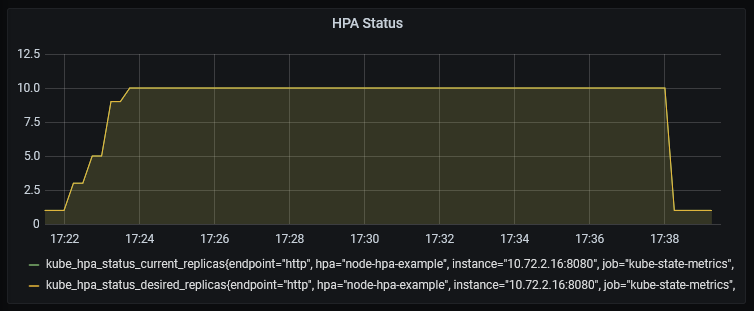
\includegraphics[width=\textwidth]{light_cpu_hpa.PNG}
  \caption{HPA által kívánt és tényleges podok száma}
  \label{light_cpu_hpa}  
\end{figure}

\Aref{light_cpu_cpu} diagramon látható a skálázott podok CPU kihasználtsága.  A kék
színű grafikon jelöli az összes pod CPU kihasználtságát, a többi ugyanezt
podokra levetítve.  Az ábráról leolvasható, hogy a teljes CPU kihasználtság
maximuma 1250m.  Ezt leosztva a replikák számával, vagyis 10-el, 125m-et
kapunk, azaz a HPA jól működött, mert az átlagos CPU kihasználtság nem ment
150m fölé. Azonban egyenként megvizsgálva a podok CPU használatát, vannak
olyan podok, amelyek elérik, és sokáig a 300m-es tartományban maradnak és
olyanok, amelyek a 100m-es tartományban maradnak.  Ebből látható, hogy a
Kubernetesben a terheléselosztás nem egyenletesen történik.

\begin{figure}[H]
  \centering
  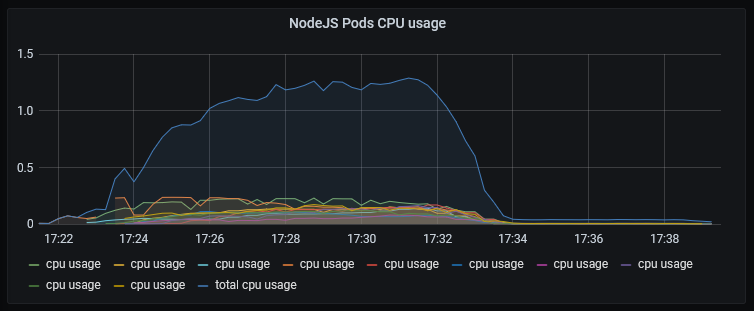
\includegraphics[width=\textwidth]{light_cpu_cpu.PNG}
  \caption{Kiszolgáló podok CPU kihaszáltsága}
  \label{light_cpu_cpu}  
\end{figure}

\Aref{light_cpu_response_time} diagramon az átlagos válaszidő látható podokra bontva.  Szinte az
összes pod kezdetben magasabb válaszidővel válaszol, ez lehet a NodeJS
Express valamilyen sajátossága miatt.  A válaszidők a teszt közepe felé egyforma
értékeket vesznek fel, majd kettő pod kivételével az összes pod válaszideje
megnő.  Ez amiatt lehet, mert a terhelésgenerálás olyan fázisba ért, ahol a
kéréseket a podok nem tudják azonnal kiszolgálni.

\begin{figure}[H]
  \centering
  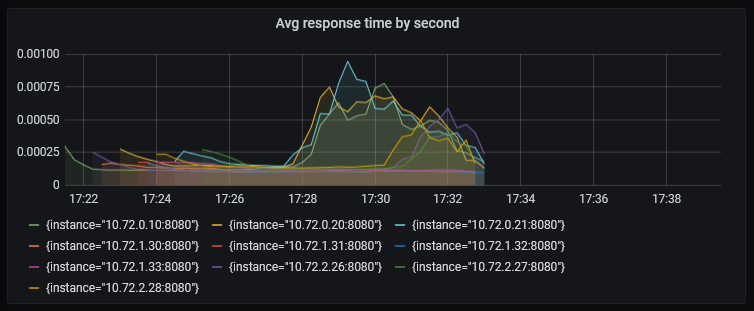
\includegraphics[width=\textwidth]{light_cpu_response_time.PNG}
  \caption{Kiszolgáló podok válaszideje 1 másodpercre vetítve}
  \label{light_cpu_response_time}  
\end{figure}

\Aref{light_cpu_response_count} diagramon az átlagos válaszok száma látható.
A zöld színű grafikon jelöli az összes pod átlagos válaszainak számát.  Ez a
diagram a teszt szerint elvárt módon növekszik a 17:28-as időpontig, majd a
válaszok arányában stagnáció áll be.  \Aref{light_cpu_response_time}
diagrammal összevetve így arra lehet következtetni, hogy a stagnáció szintén
a podokra nehezedő terhelés következménye.

\begin{figure}[H]
  \centering
  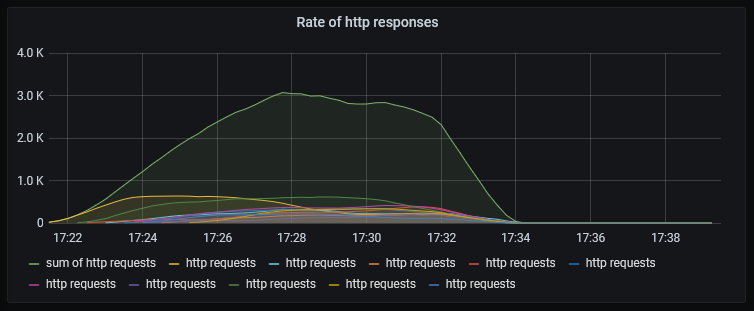
\includegraphics[width=\textwidth]{light_cpu_response_count.PNG}
  \caption{Kiszolgáló podok válaszainak száma 1 másodpercre vetítve}
  \label{light_cpu_response_count}  
\end{figure}

\subsubsection{Skálázás az átlagos válaszok számának függvényében}
\label{secsec:custom_scaling}

Az egyedi metrikára az átlagos válaszok számát választottam.  Az előző
mérésből \aref{light_cpu_response_count} ábra alapján az átlagos válaszok
számának küszöbét a HPA-ban 500-ra állítottam.

A teszt lefutásához ugyanazokat a diagramokat hoztam létre, mint a CPU alapú
skálázásnál \aref{secsec:cpu_scaling} fejezetben.

\Aref{light_custom_hpa} ábrán a HPA által kívánt és tényleges podok száma
látható.  Összevetve \aref{light_cpu_hpa} ábrával a podok száma sokkal
lassabban növekszik, és csak hat podot használ ki a maximális tízből.

\begin{figure}[H]
  \centering
  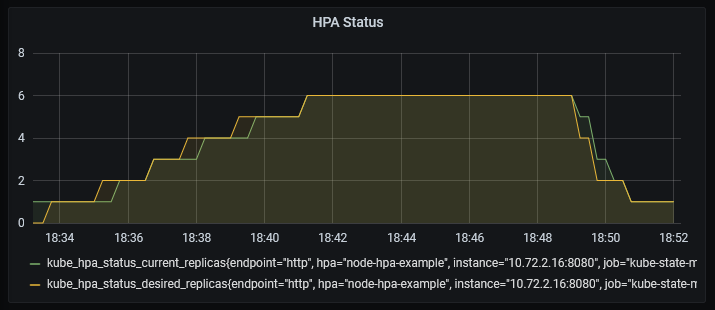
\includegraphics[width=\textwidth]{light_custom_hpa.PNG}
  \caption{HPA által kívánt és tényleges podok száma}
  \label{light_custom_hpa}  
\end{figure}

\Aref{light_custom_cpu} ábrán látható CPU kihasználtságot összevetve
\aref{light_cpu_cpu} ábrán látható CPU kihasználtsággal látható, hogy az
egyéni metrikákkal történő skálázásnál a CPU kihasználtság sokkal jobban
követi a tesztben is definiált lineáris terhelést, valamint a CPU terhelés kisebb, mint a
CPU alapú slálázás esetében.

\begin{figure}[H]
  \centering
  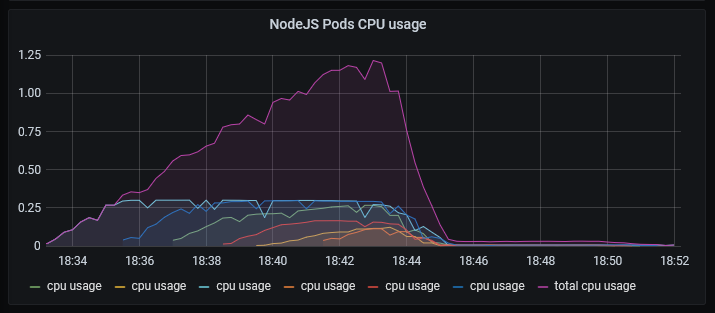
\includegraphics[width=\textwidth]{light_custom_cpu.PNG}
  \caption{Kiszolgáló podok CPU kihaszáltsága}
  \label{light_custom_cpu}  
\end{figure}

\Aref{light_custom_response_time} ábrán látható válaszidőket összevetve
\aref{light_cpu_response_time} ábrán látottakkal, a válaszidők a teszt elején
még nagyjából megegyeznek, a 0.1-0.2 ms tartományba esnek.  Az egyéni
metrikákkal történő skálázásnál is megnőnek a válaszidők a teszt végére,
azonban ez sokkal később történik meg, és csak két podnál emelkedik
számottevően.

\begin{figure}[H]
  \centering
  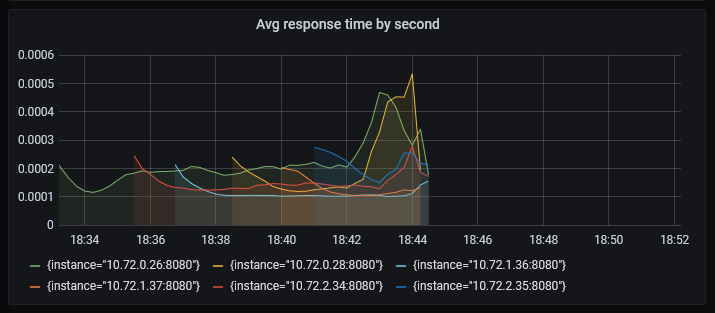
\includegraphics[width=\textwidth]{light_custom_response_time.PNG}
  \caption{Kiszolgáló podok válaszideje 1 másodpercre vetítve}
  \label{light_custom_response_time}  
\end{figure}

\Aref{light_custom_response_count} ábrán is megfigyelhető
\aref{light_custom_cpu} ábrához hasonló lineáris növekedés, azaz a válaszok
átlagos száma is jól követi a tesztben definiált terhelés növekedését.
Azonban itt is megfigyelhető, hogy mivel a HPA a podok válaszainak egy
másodpercre vetített számának átlagát veszi, a podok válaszainak száma nem
lesz 500 alá szorítva.

\begin{figure}[H]
  \centering
  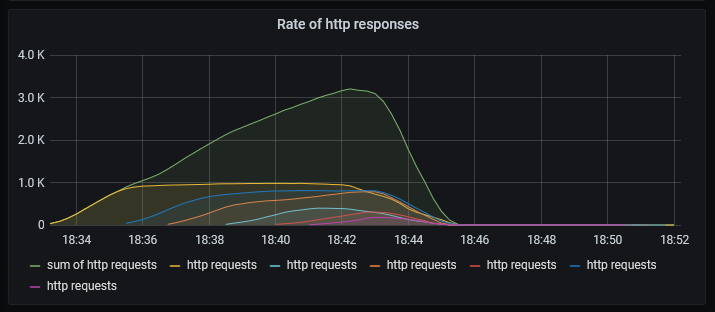
\includegraphics[width=\textwidth]{light_custom_response_count.PNG}
  \caption{Kiszolgáló podok válaszainak száma 1 másodpercre vetítve}
  \label{light_custom_response_count}  
\end{figure}

\subsection{Összefoglalás}
\label{sec:osszefoglalas}

\Aref{secsec:cpu_scaling} részben bemutattam egy CPU alapú skálázást és
\aref{secsec:custom_scaling} részben egy HTTP válaszok átlagos száma alapján
történő skálázást.  A tesztek futásakor kapott metrikák azt mutatták, hogy a
válaszok átlagos száma alapján történő skálázás CPU kihasználtságban és
válaszidőben is jobb eredményeket produkált, mint a CPU alapú skálázás.  A
mérésekből az a következtetés vonható le, hogy a tényleges terhelést leíró
metrikákat használva jobb kihasználtságot és jobb metrikus adatokat lehet
kapni az erőforrás alapú skálázáshoz képest.

\newpage
 
%==================================================================
\section{Irodalom, és csatlakozó dokumentumok jegyzéke}
\label{sec:irod-es-csatl}

\begin{thebibliography}{9}
\label{sec:tanulm-irod-jegyz}

\bibitem{web} \emph{Tájékoztató a Műszaki Informatika Szak önálló
    laboratórium tantárgyainak 2008/9. tanév I. félévi lezárásáról a
    BME TMIT-en (VITMA367, VITMA380, VITT4353, VITT4330),}
  \url{http://inflab.tmit.bme.hu/08o/lezar.shtml}, szerk.: Németh Felicián,
  2008. november 5.

\bibitem{wikipedia} Wikipedia contributors, \emph{Wikipedia:Academic
    use}, Wikipedia, The Free Encyclopedia, 2011 Nov 11.  Available
  from: \\ \url{http://en.wikipedia.org/w/index.php?title=Wikipedia:Academic\_use\&oldid=460041928}

\end{thebibliography}

%==================================================================
\subsection{A csatlakozó dokumentumok jegyzéke}
\label{sec:csat-irod}

\end{document} 

%%% Local Variables: 
%%% mode: latex 
%%% TeX-master: t 
%%% End:

